
\subsection{Data qubit displacement}
Yo

[BELOW LIES OLD CRAP]\\
\\

The effect of displacement of the data qubits from the ideal was investigated. Ideally the data qubits would be in a square lattice of spins precisely $D = \SI{400}{\nano\metre}$ apart, but due to inaccuracies in dopant spin placement each qubit will have small displacements from the ideal lattice position.

This is modelled by generating a uniform random displacement within a given pillbox $xy$-radius and $z$-height. Simulations from the original paper show $\textrm{radius} = \textrm{height} = \SI{6}{\nano\metre}$ to be a threshold for this scheme. The phase accumulated over 25 runs for this pillbox size is plotted as a histogram in fig.\@ \ref{fig:DisplacementPhaseHistogram}, showing a maximum phase error of $\tfrac{\pi}{4}$ for these runs. 



The effect of displacements in the $x$-$y$ plane and the $z$-axis are significantly different in magnitudes, due to the $\tfrac{1}{d^3}$ term in the Hamiltonian being most strongly affected by $z$ displacements. This effect was investigated by artificially setting displacements in these directions.

Fig.\@ \ref{fig:zoffset} shows changes in accumulated phase due to $z$-displacements. The first 2 qubits are displaced \SI{4}{\nano\metre} down, slowing the evolution and giving a noticeable phase error after half a cycle. However, qubit 4 is displaced \SI{3}{\nano\metre} upwards, reducing $d$ and resulting in faster evolution. The effect is a small phase error from the ideal $2\pi$.

Fig.\@ \ref{fig:inwarddisplacement} shows the effect of displacements in the $x$-$y$ plane. For this run, all data qubits were displaced \SI{10}{\nano\metre} inwards with respect to the circular motion. The phase error on each individual qubit is then less than that produced by the \SI{3}{\nano\metre} $z$-displacement of fig.\@ \ref{fig:zoffset}, showing the smaller sensitivity to displacement in the $x$-$y$ plane, though the overall error after all 4 qubits is greater as in the $z$-direction, +$z$ and --$z$ errors cancel out somewhat, whereas $xy$ displacement errors will always slow the evolution.

\begin{figure}[h]
	\centering
	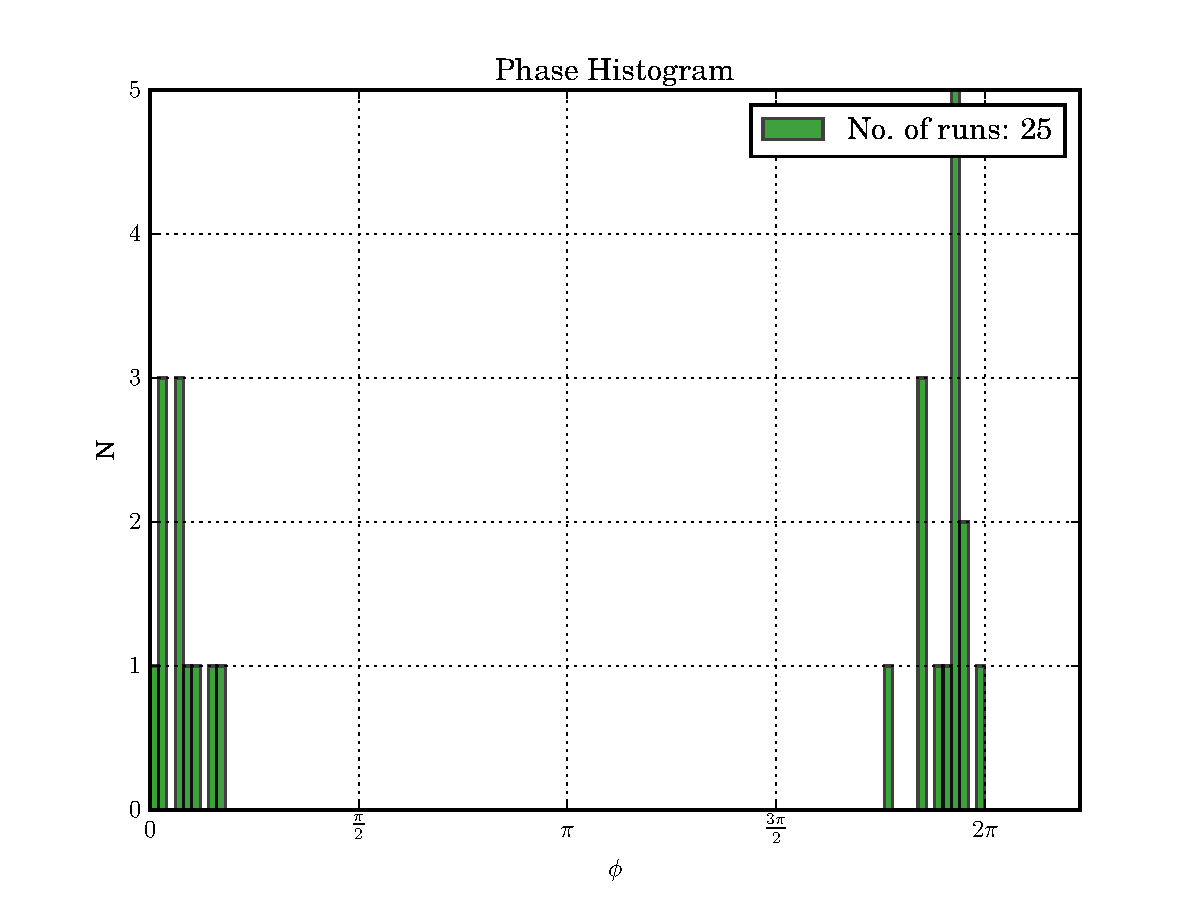
\includegraphics[width=\textwidth]{../Figures/Displacement_phase_histogram.pdf}	
	\caption{Phase errors over 25 runs as a result of randomly generated data qubit displacements within a pillbox of half-height \SI{3}{\nano\metre} and radius \SI{6}{\nano\metre}. These values are a threshold for the proposed scheme.}
	\label{fig:DisplacementPhaseHistogram}
\end{figure}

\begin{figure}[H]
	\subfloat[]{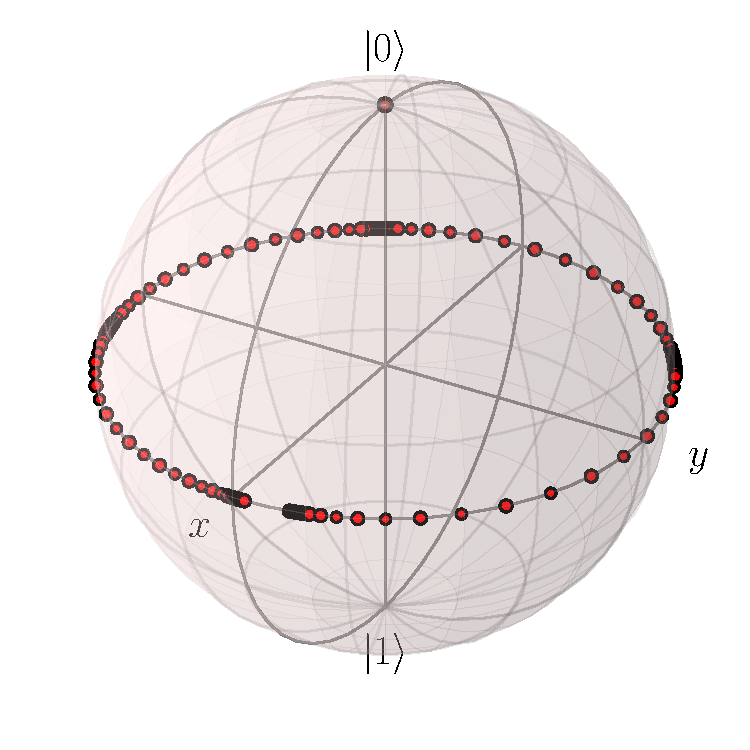
\includegraphics[width=0.49\linewidth]{../figures/z_offset.pdf} \label{fig:zoffset}}
	\subfloat[]{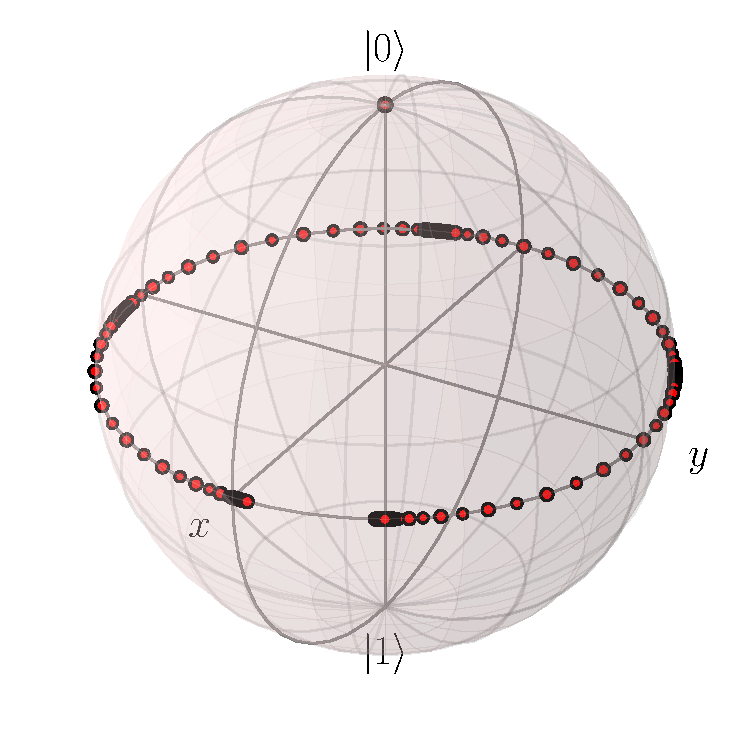
\includegraphics[width=0.49\linewidth]{../figures/10nm_displacement_inward.pdf} \label{fig:inwarddisplacement}}
	\caption[oddeven]{(a) Evolution of probe qubit with data qubit displacement in the Z direction. 1st and 2nd qubits are displaced \SI{4}{\nano\metre} down, slowing the evolution, the 4th is displaced \SI{3}{\nano\metre} up with a resultant increase in phase accumulated. The overall deviation from $2\pi$ is small as a result. (b) Phase accumulated when all 4 data qubits are displaced \SI{10}{\nano\metre} towards the centre of the circle. Other directions of \SI{10}{\nano\metre} displacements result in similar phase deviations.}
	\label{fig:overall_displacement}
\end{figure}


